\chapter{CERN, the LHC and LHCb}
\label{CERN_LHC_LHCb}


The European Organisation for Nuclear Research (CERN) was founded in 1954 and began with 12 member states as a organisation to encourage European collaboration and the study of nuclear physics. Since it's foundation the collaborative nature of CERN allowed for large-scale expensive experiments and machines to be built. The Proton Synchrotron was CERN's flagship accelerator, operational in 1959 it had a circumference of 628~m and accelerated protons to 25~GeV, the highest energy at that time. Now 62 years since it's foundation CERN has grown to include 21 member states \footnote{about the other types of countries involved.} and is still at the forefront of high energy physics research. CERN’s latest accelerator, the Large Hadron Collider (LHC), is most energetic particle accelerator ever built, with a 27km circumference the LHC was designed to protons at~14 TeV. \textit{(make sure to mention ions in the LHC section and explain how their energy is limited by the magnets which get protons to 14 TeV in the LEP tunnel). }  This chapter shall discuss the LHC and the LHC beauty experiment, one of the experiments that uses collisions provided by the LHC.

Not sure about the above but;
%%%%%%%%%%%%%%%%%%%%%%%%%%%%
Here there will be some words introducing this Chapter, I think they should be focused on what makes a nice clear introduction not about the cool facts that I have learnt. I think that this part should be done last and should include a little information about the LHC and LHCb and then explain what this chapter is about. My thesis is about data from the LHCb experiment no about how cool CERN is.

Prehaps add in above where the sources where I got most of the information are from!

\section{The LHC}
\label{LHC}

Rough ideas
%%%%%%%%%%%%%%%

The LHC was designed to cllide protons at 14 TeV. It collides lead-ions too but these are irrelevant to my thesis. The LHC accelterated and collides protont and ipons and it has 2 beams that go in oposite directions.


It starts with protons from hydrogen whccih are accelerated through a chain of past CERN accelerators adapted to feed the LHC. 

The protons are around 450 GeV when they are put into the LHC. They are delivered in bunches. THe LHC then accelerates these beams of proton bunches using RF cavities, bendin the beam around it's ring with dipole magents up to the desirerd energu. Once they have made it, the numches are quite spread out so need to be focued sing quadroploe magnets before they are collided at the 4 intereaction points. Prehaps some details about fills of the LHC? Look here is a picture of the accelerator chain that feeds the LHC. 

As well as the energy as an important charteristic of a collider - because the cross-section to produce various particles increases with energy, the luminoscity  is also well important. The instantaneous luminoscity is given here and the parameters mean some interesting things. The luminoscity is proportianol to the collision rate. The parameters can be controlled by the magents to suit the different needs of the experiments. For example ATLAS and CMS use all possible luminoscity which decreases with a fill, where as LHCb operates at a lower luminoscity which is made constant through adjustments to the bunch shapes during a fill. Look here is a cool graph that shows all the things.

There are 7 experiemnts on the LHC that make used of these collisions. CMS and ATLAS are general purpose detectors which were designed to search for the Higgs and identify NP particles which are not in the SM. ALICE uses heavy ion collisions to study quark-gluon plasma. LHCf, TOTEM and MODAL fo some other things. The final experiment LHCb collects data that is used in this thesis and will be explained soon.

The LHC began properly in 2010 and ran in 2012 taking data at 7TeV and 8TeV, there was then a long shut down and various things were done. In 2015 data taking started up again, and is still on going, at the higher energy of 13TeV. The nice table here shows the energy the LHC opereated at each year and the integrated luminoscity collected by LHCb. (Not sure if this should go here or somewhere else, leave here for now).



So overall this plan seems to be;
%%%%%%%%%%%%%%%%%%%%%%%%%%%%%%%%%
1> The LHC is a synchrotron to collide protons at 14 TeV (and ions)
2> This is how the LHC gets it's protons and accelerates them (maybe mention the bunch spacing too?)
3> Now only is energy important but so is luminoscity and here is how we get that
4> Here are the experiments that are on the LHC - see they are different
5> This is what the LHC has done since 2010 and here are the numbers of energy and luminoscity for LHCb 

.1
%%%%%%%%%%%%%%%%%%%%%%%%%%%%%%%%%%%%%%%%%%%%%%%%%%%%%%%%%%%%%%%%%%%%%%%%%%%%%%%%%%%%%%%%%%%%%%%%%%%%%%%%%%%%%%%%%%%%%%%%%%%%%%%
So lets now accumulate some facts 
%%%%%%%%%%%%%%%%%%%%%%%%%%%%%%%%%
1> The LHC is a synchrotron to collide protons at 14 TeV (and ions)
a synchrotron 
The LHC was conceived in 1980.
It was built in the LEP tunnel with a circumference of 27km. (To operate at 14TeV is needed 8.3T magnets to bend the beams.)
The LHC can also collide lead ions can get to an energy of 2.76 TeV per nucleon due to the 8.3T magnets.
Protons travel in oposite directions around the ring in seperate vacuum chambers and are bent by dipole magnets.
Protons are brought to collide in 4 seperate places.
The products of these collisions are recoreded by some experiments.

Sentences
%--------
The LHC is a proton synchrotron that was designed to accelerate and collide two beams of protons travelling in oposite directions up to a center-of-mass energy of 14~TeV. Although operation of the LHC began in 2010 it is yet to reach design energy. The purpose of the LHC is to provide high energy proton collisions, the products of which are used for precision tests of the Standard Model (SM) and to search for new physics particles that go beyond the scope of the SM. There are four interaction points on the LHC ring where the beams are brought to collide, at these points various experiments detect and study the products of these collisions. The LHC can also accelerate lead-nuclei up to an energy of 2.76~TeV per nucleon, but it is only the products from proton collisions that are the topic of this thesis.


The protons for the LHC are supplied by hydrogen .... Bring on point 2.

.2
%%%%%%%%%%%%%%%%%%%%%%%%%%%%%%%%%%%%%%%%%%%%%%%%%%%%%%%%%%%%%%%%%%%%%%%%%%%%%%%%%%%%%%%%%%%%%%%%%%%%%%%%%%%%%%%%%%%%%%%%%%%%%%%
So lets now accumulate some facts 
%%%%%%%%%%%%%%%%%%%%%%%%%%%%%%%%%
2> This is how the LHC gets it's protons and accelerates them (maybe mention the bunch spacing too?)

Protons come for hydorgen atoms in a gas they are ionised to get the protons
First Linac2 accelerated to 50MeV Proton Synchrotron Booster (PSB) -4 parallet accelerator ringe increase to 1.4 GeV
PS divided into bunches and up to 25? GeV
Super PRoton Synchrotron up to 450 GeV theen they are injected into the LHC. At injection the proton bunches are divided into two beams travelling in oposite directions.
1232 dipole magnets to keep protons going in a circle increased up to 8.3T as beams go up to 7TeV. Magents are at 1.9K. 15m in length.
Quadropole magnets focus the beams. 392 5-7m in length
16 super conducting Radio frequency cavities accelerate the protons (8 per beam), cavities ensure protons going to fast get smaller acceleration and slow protons get a higher acceleration.
Parts of the chain did cool physics stuff in the past.
LHC designed to make bunches seperated by 25ns but Run 1 had only 50 ns and 2015 saw 25ns - (I've not mentioned when it has run yet prehaps put details of the running all together at the end)
bunch crossing rate is 40 MHz
2808 bunches per beam with > 10^{11} protons in a bunch but there could be 3600 but there are not because of transfer and injection, include these numbers because they are relevant for luminoscity.
Design luminoscity is 10^34cm-2s-1
The existing accelerators were upgraded to give the needed bunch intensities and emmittances.
The revolution frequency for beams is 11.245 kHz.


Sentence ideas - this is what I originally has
%--------------------------------------------
It starts with protons from hydrogen whccih are accelerated through a chain of past CERN accelerators adapted to feed the LHC. 

The protons are around 450 GeV when they are put into the LHC. They are delivered in bunches. THe LHC then accelerates these beams of proton bunches using RF cavities, bendin the beam around it's ring with dipole magents up to the desirerd energu. Once they have made it, the numches are quite spread out so need to be focued sing quadroploe magnets before they are collided at the 4 intereaction points. Prehaps some details about fills of the LHC? Look here is a picture of the accelerator chain that feeds the LHC.

I think that the order here is nice.



The protons for the LHC originate from hydroden atoms in a gas, the gas is ionised to strip away the electrons and the protons are accelerated through a chain of particle accelerators of increasing energy before being injected into the LHC. The chain of accelerators, shown in Fig.~\ref{fig:accelerator_chain}, consists of existing accelerators that have been used in various experiments through the second half of the last century and have been upgraded to meet the requirements needed for providing protons for the LHC. 
The protons leave the chain of accelerators with of energy of 450 \gev per proton and in bunches of  >$10^{11}$, as the bunches injected into the LHC they are split into two opositely circulating beams.
The LHC accelerates the protons to the desired center of mass energy using supercooled Radio Frequency cavities for acceleration and superconducting dipole magnets to bend the beams around the ring. 
%The design configuration for the beams is to have 2808 bunches per circulating beam with 25~ns between each bunch, 
Then bunches are focused using quadrupole magnets before being brought to collide at 4 interaction points with a bunch crossing rate of 40~MHz. 

The energy at which the bunches are collided determines the production cross-section of different particles

\begin{figure}[htbp!] 
\centering    
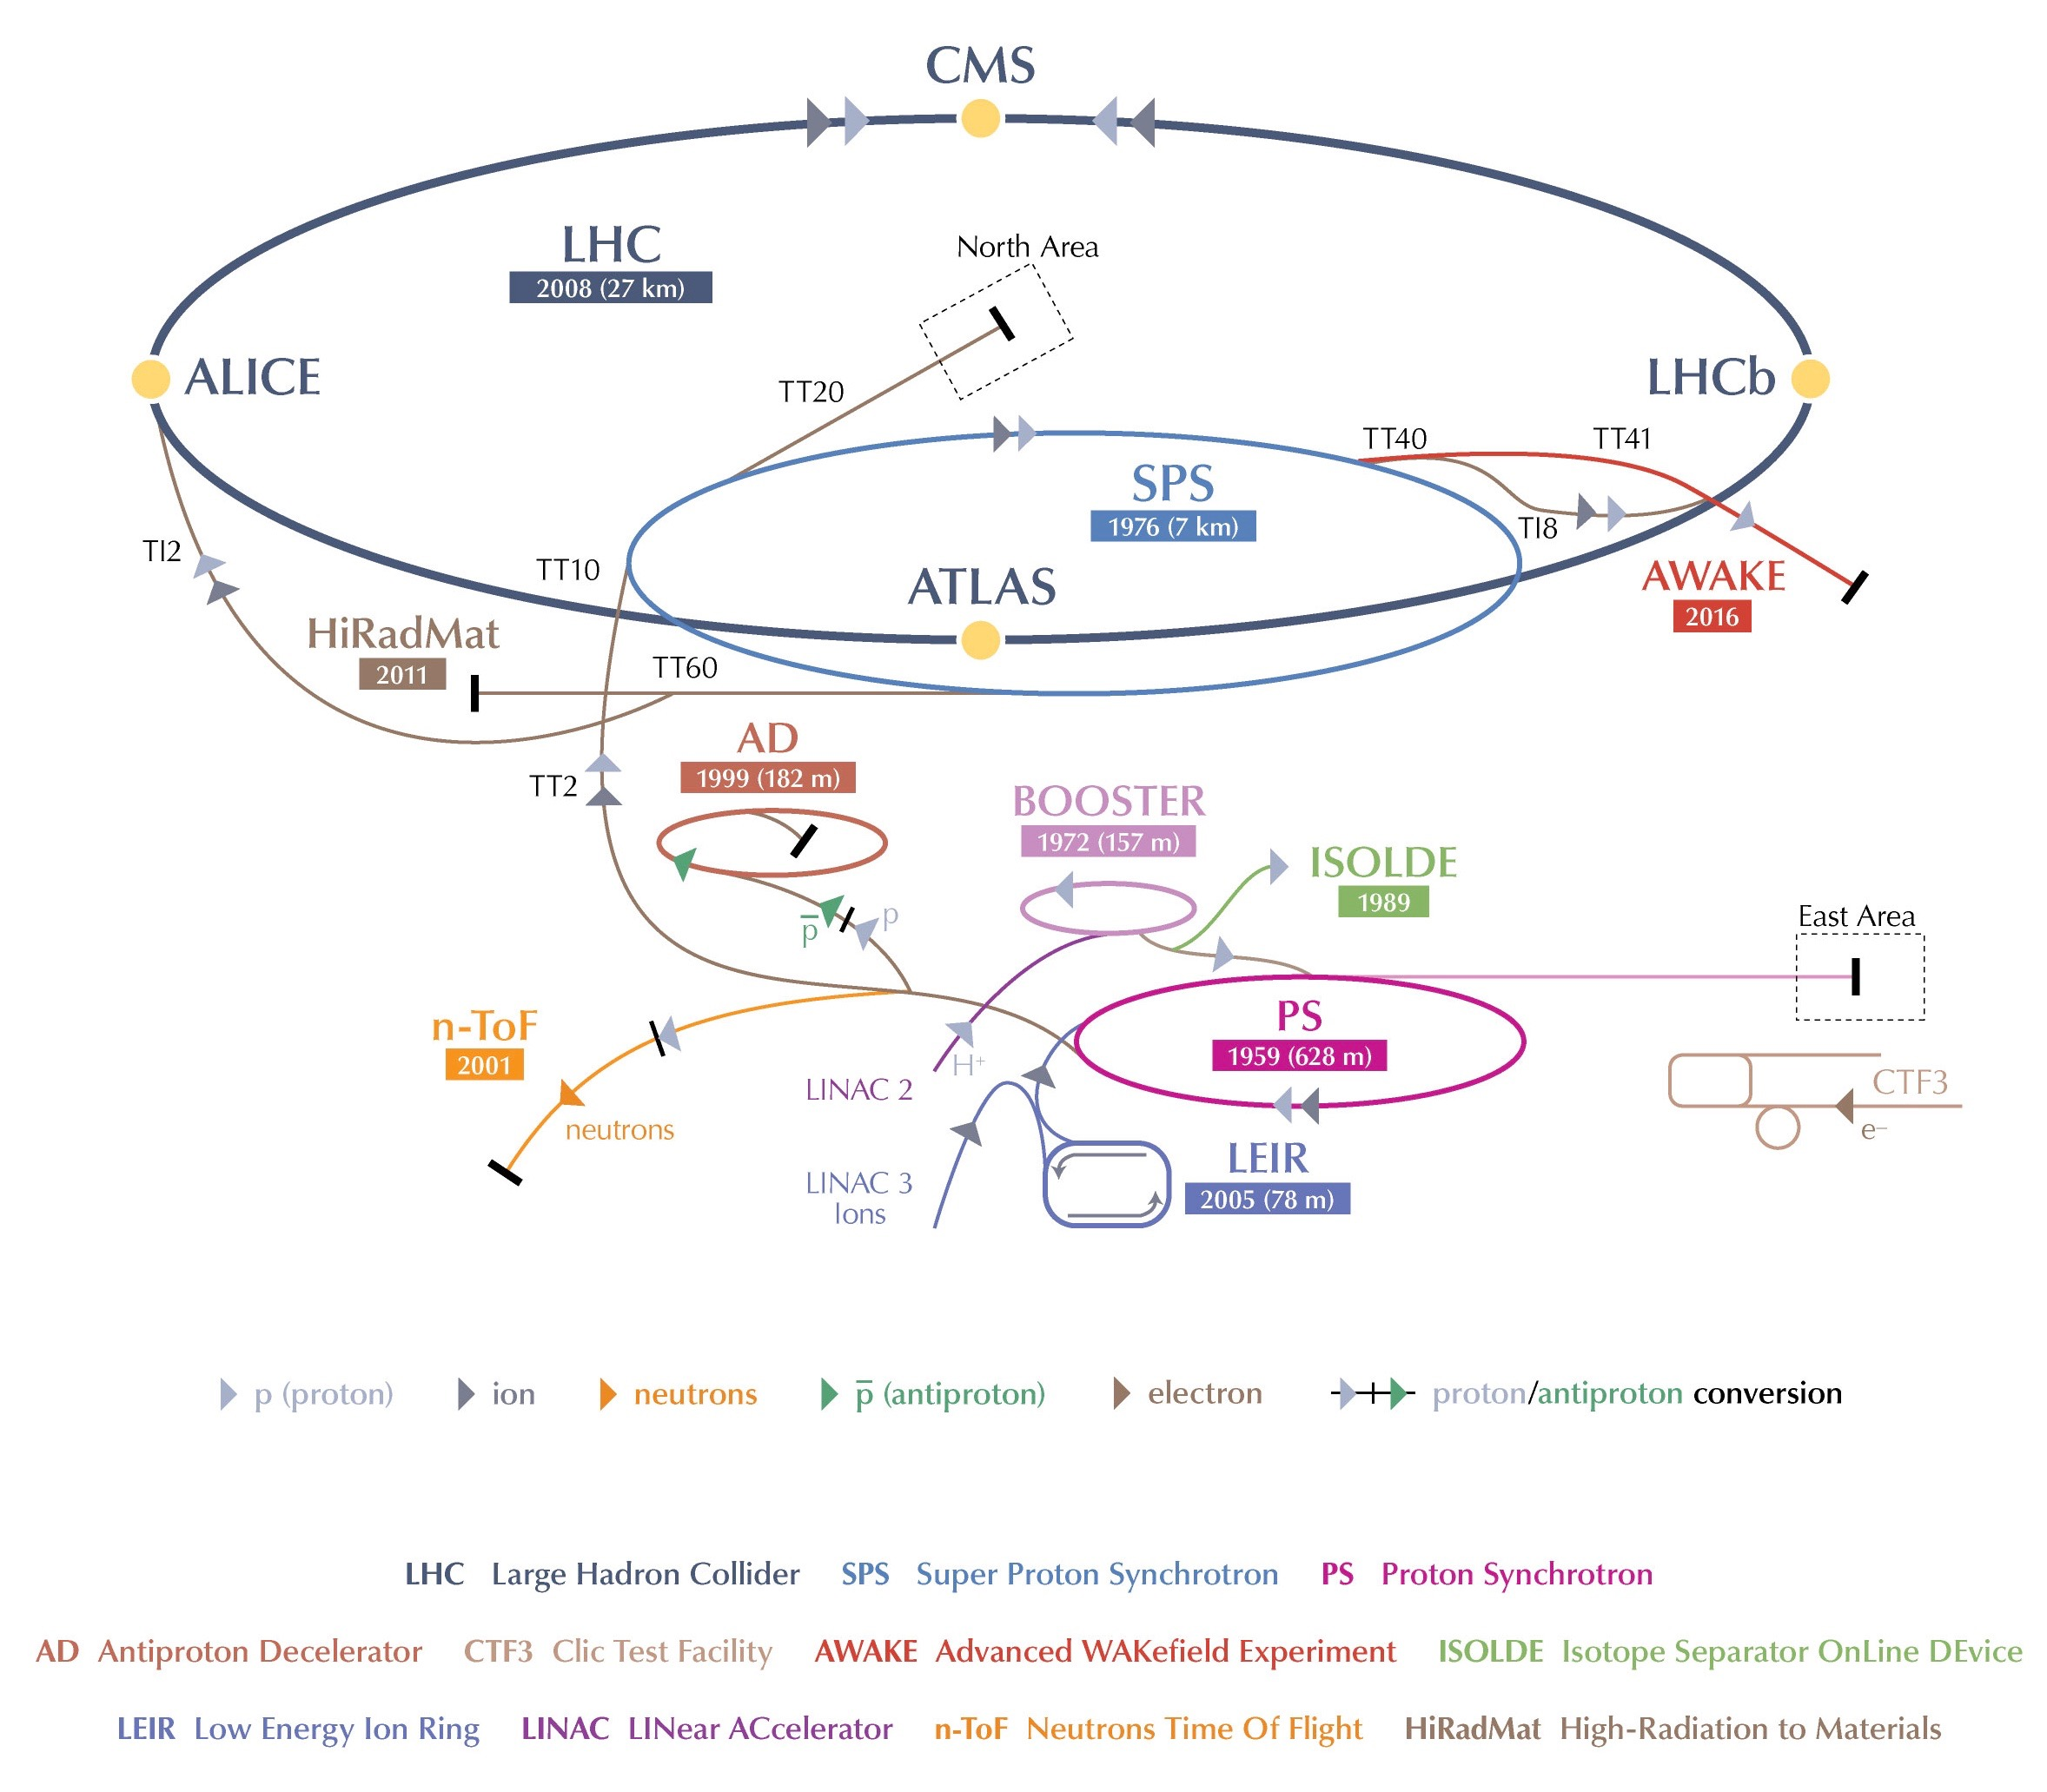
\includegraphics[trim = 125mm 2mm 125mm 90mm, clip, width=1.0\textwidth]{accelerator_complex.jpg}
\caption{The accelerator complex at CERN. The chain of accelerators used by the LHC consists of the Linac 2 accelerating protons to 50\mev, the Proton Synchrotron Booster accelerating protons to 1.4\gev, the Proton Synchrotron accelerating protons to 25\gev and creating the desired spacing between proton bunches then finally the Super Proton Synchrotron accelerating protons to 450\gev. Source: CERN.}
\label{fig:accelerator_chain}
\end{figure}

.3
%%%%%%%%%%%%%%%%%%%%%%%%%%%%%%%%%%%%%%%%%%%%%%%%%%%%%%%%%%%%%%%%%%%%%%%%%%%%%%%%%%%%%%%%%%%%%%%%%%%%%%%%%%%%%%%%%%%%%%%%%%%%%%%
So lets now accumulate some facts 
%%%%%%%%%%%%%%%%%%%%%%%%%%%%%%%%%
3> Now only is energy important but so is luminoscity and here is how we get that
It would be nice here to have a plot of the integrated luminoscity delivered to LHCb over 2011 - 2016.
Luminoscity is a measure of the collision rate
design liminoscity is 10^34cm-2s-1
The lunminoscity is reached through numbers of bunches and revolution frequency/25ns.
Magnets focus the beams into the shape required for the delivered luminoscity.
Difference between instananeous and integrated luminoscity,
Can also have luminoscity in terms of mu.
Experiments can focus/defocus the beam to get the luminoscity they require.
Instantaneous lumi can be integrated over time and this is how we get a measure of how much data is recorded.
The maximum instaneanous lumi decreases over time as the number of protons in the bunches reduces. LHCb uses luminoscity leveling so that it gets the same luminoscity all the time.
Luminoscity is a measure of the number of protons crossing a unit area per unit time.
Energy allow new effects to be produced but luminoscity is also important because if show the number of crossing and the number of events in a process pre second is N = L.sigma where sigma is the production cross section for a praticular process for if sigma is low we need high luminoscuty. (What is the production cross section of Bs and Bd mesons? Surely high but we just have a low BF.)


The number of events produced as the beams collide for a particular process pre second is given by

N = L . sigma

where L is the instantaneous luminoscity and sigma the production cross section for the process. 

The prodcution cross-section for difference particles depends on the CoM energy of the collisions, the high energies the LHC can reach at allows the production of particles not accessible at past colliders. 
But in order to get a large number of interesting events the instantaneous luminoscity is also important. 

The instantaneous lunimoscity is a meaure of how many collisision occur per second, it is given by

\begin{equation}
\mathcal{L} = \frac{N^{2} f n_{b}}{\mathcal{F}}.
\label{eq:inst_lumi}
\end{equation}

where $N$ is the number of protons per bunch, $n_{b}$ the number of bunches per beam, $f$ the bunch revolution frequency and $\mathcal{F}$ contains information about the beam geometry. The LHC is designed to operate at an instantaneous luminoscity of $10^{34}$ cm$^{-2}$s$^{-1}$, in order to reach this luminoscity the LHC can have 2808 bunches per beam and a revolution frequency for beams is 11.245 kHz leading to a seperation of 25 ns between bunches. The luminoscity delivered at each interaction point can be tuned by the quadrupole magnets altering the shape of each bunch.


The high energies that the LHC operates at allows the production of particles not accessible at past colliders (eg the Higgs and would allow the search for heavy BSM particles). However in order to produce a large number of these particles the LHC the number of proton interactions per bunch crossing needs to be large. The luminoscity of a collider is a measure of the collision rate

The production of particles increases with energy therefore the high energies at the LHC could allow for greater number of particles to be produced or new particles.










But in order to get a large number of interesting events the instantaneous luminoscity is also important. 


The CoM energy of a collider is an important measure of it's preformance as it dictates what particles can or could be produced in collisions but another important measure of collider performance is the instantaneous luminoscity a collider can provide. The instantaneous luminoscity, $\mathcal{L}$, is a meaure of how many collisision occur per second, it is given by

\begin{equation}
\mathcal{L} = \frac{N^{2} f n_{b}}{\mathcal{F}}.
\label{eq:inst_lumi}
\end{equation}

where $N$ is the number of protons per bunch, $n_{b}$ the number of bunches per beam, $f$ the bunch revolution frequency and $\mathcal{F}$ contains information about the beam geometry. The LHC is designed to operate at a maxiumum instantaneous luminoscity of $10^{34}$ cm$^{-2}$s$^{-1}$, in order to reach this luminoscity the LHC can have 2808 bunches per beam and a revolution frequency for beams is 11.245 kHz leading to a seperation of 25 ns between bunches. The higher the luminoscity, the more collisions happen in a second and the more particles will be produced, this can either be advantageous or disadvantageous depending on what physics process is being studied and the detector design that recors the collisions. Therefore luminoscity delivered at each interaction point can be tuned by the quadrupole magnets by altering the shape of each bunch for the experiments at each point.



\section{The LHCb Experiment}
\label{LHCb}
